\documentclass{article}
\usepackage{amsmath,amssymb,tikz}
\newcounter{question}
\setcounter{question}{0}
\begin{document}

\newcommand\Que[1]{%
   \leavevmode\par
   \stepcounter{question}
   \noindent
   \thequestion. Q) #1\par}

\newcommand\Ans[2][]{%
    \leavevmode\par\noindent
   {A) \textbf{#1}#2\par}}

\Que{
   Volume of region enclosed by $y=8x^3, y=0, x=1$ about $x=2$\\
}
\Ans{

   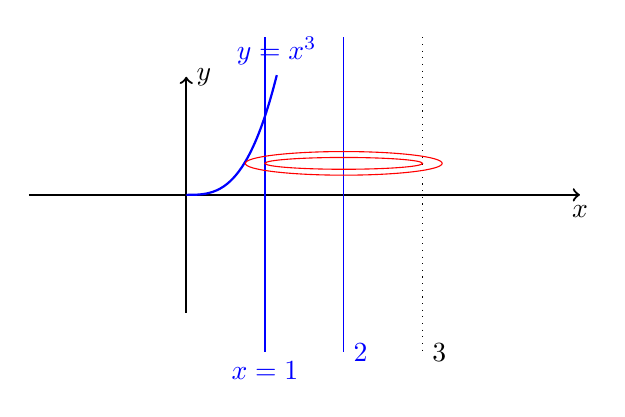
\begin{tikzpicture}[smooth,scale=1]
      \draw[thick,->] (-2,0) -- (5,0) node[below] {$x$};
      \draw[thick,->] (0,-1.5) -- (0,1.5) node[right] {$y$};

      \draw[blue,thick,domain=0:1.15] plot (\x,{\x*\x*\x}) node[above] {$y=x^3$};

      \draw[blue,thin] (1,2) -- (1,-2) node[below] {$x=1$};
      \draw[blue,thin] (2,2) -- (2,-2) node[right] {$2$};
      \draw[dotted] (3,2) -- (3,-2) node[right] {$3$};

      \draw[red] (2,0.4) ellipse (1.25cm and .15cm);
      \draw[red] (2,0.4) ellipse (1cm and .075cm);
   \end{tikzpicture}\\

   Since the size of the ``ring'' is a function of $y$ 
   (think sliding it up and down to change its size), 
   we convert the original function in terms of $y$. 
   In other words,\\

   \begin{equation}
      x = f(y) = \frac{\sqrt[3]{y}}{2}
   \end{equation}\\

   This ``ring'' has 2 radii: the outer one: $R$ 
   and the inner one: $r$\\

   We see that $r=1$ (the distance between $x=1$ and $x=2$)\\

   $R$, however, is the distance between $x=2$ and $f(y)$. Using (1) above:\\

   $ R=2-\frac{\sqrt[3]{y}}{2} $\\

   The area of this ring:\\
   
   $ A(y) = \pi{R}^2-\pi{r}^2 $ \\

   $ = \pi(2-\frac{\sqrt[3]{y}}{2})^2 - \pi{(1)}^2 $\\

   $ = \pi \left[ (\frac{4-\sqrt[3]{y}}{2})^2 - 1 \right]
   = \pi \left[ (\frac{16+{y}^{2/3}-8{y}^{1/3}}{4}) - 1 \right] $\\
   
   $ = \frac{\pi}{4} \left[ 16 + {y}^{2/3} - 8{y}^{1/3} - 4 \right]
   = \frac{\pi}{4} \left[ 12 + {y}^{2/3} - 8{y}^{1/3} \right] $\\

   The volume of the solid generated by the curve is 
   the integration of this ``ring'' w.r.t $dy$,
   calculated in the range $[0,8]$
   (the extremes of the curve where it intersects with the limiting lines).\\
   
   $ V = \int_{0}^{8}{A(y)} dy $\\

   $ = \int_{0}^{8}{\frac{\pi}{4} \left[ 12 + {y}^{2/3} - 8{y}^{1/3} \right]} dy $\\

   $ = \frac{\pi}{4} \int_{0}^{8}{\left[ 12 + {y}^{2/3} - 8{y}^{1/3} \right]} dy $\\
   
   $ = \frac{\pi}{4} \left[ 12y + \frac{{y}^{5/3}}{5/3} - \frac{8{y}^{4/3}}{4/3} \right]_{0}^{8} $\\
   
   $ = \frac{\pi}{4} \left[ 12(8) + \frac{{(8)}^{5/3}}{5/3} - \frac{8{(8)}^{4/3}}{4/3} \right] $\\

   $ = \frac{\pi}{4} \left[ 96 + \frac{32}{5/3} - \frac{384}{4/3} \right] $\\

   $ = \frac{\pi}{4} \left[ 96 + \frac{96}{5} - 96 \right] $\\
   
   $ = \frac{\pi}{4} (\frac{96}{5})
   = \boxed{\frac{24\pi}{5}} $\\
}
\end{document}